
\section{Forrester diagram}
The time scope selected for the simulation was 4 years (48 months for Vensim), this is due to the fact that the exchange market, in general, is highly volatile and unpredictable; it would be a mistake to attempt a larger simulation. Besides, for the kind cryptocurrency that is being modeled, the price tends to increase in a short period of time. The complete Forrester Diagram is shown in Figure \ref{img:forrester}.
\begin{figure}[ht]
	\centering
    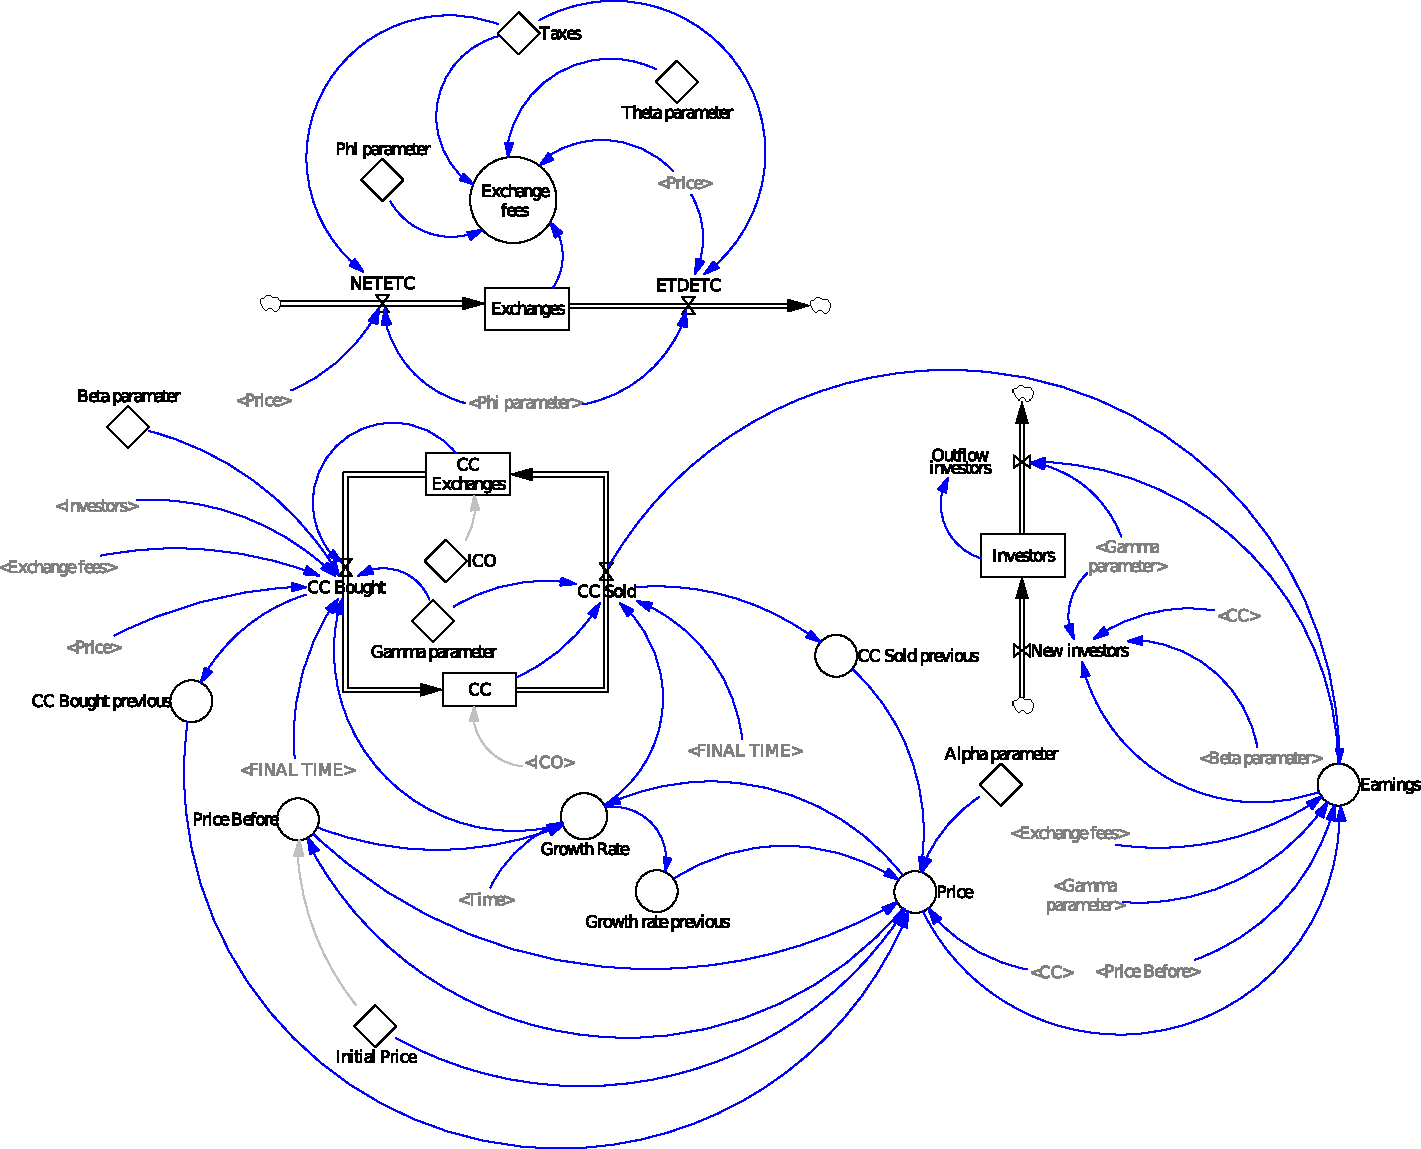
\includegraphics[scale=0.6]{files/ForresterDiag.pdf}
    \caption{Forrester diagram for cryptocurrency exchange market.}
    \label{img:forrester}
\end{figure}

It is important to highlight that, in comparison with the dynamic hypothesis, the Forrester Diagram has a considerably more variables; this is due to the fact that, during the construction of aforementioned diagram, we considered more calculations and relations between than the variables defined in first place. Although, the dynamic hypothesis has the general system behavior. This diagram was developed in Vensim.
